\section{Metodologia}

\subsection{Mudança de Fase em Balão de Vidro}
Foi utilizado um balão de vidro acoplado a um cilindro capilar aberto de mesmo material. O balão foi submetido a aquecimento e, em seguida, a ponta do ciléndro foi submersa em água. A entrada de água no interior do balão foi observada ao longo do processo de resfriamento do mesmo. A \cref{fig:balão} mostra o experimento realizado.

\begin{figure}[H]
\centering
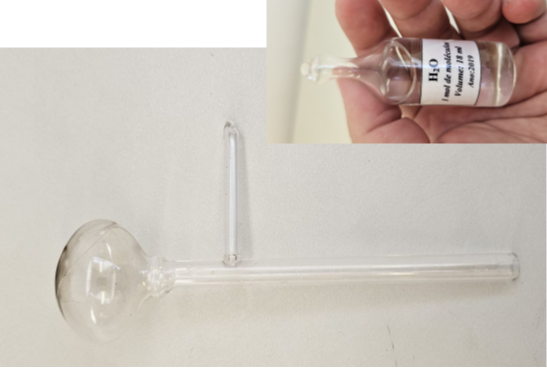
\includegraphics[width=0.30\linewidth]{fig/balao.png}
\caption{Sistema experimental com balão de vidro acoplado a um cilindro e uma haste transparente para auxiliar o manuseio do equipamento. No canto superior direito, uma frasco cheio representando um mol de água Fonte: fotografia registrada pelo monitor da disciplina.}
\label{fig:balão}
\end{figure}

\subsection{Pistão com Movimento por Sopro}
A montagem experimental consistiu em um tubo acoplado a uma câmara contendo um pistão móvel conectado a um disco. Um dos participantes soprou no tubo, o que provocou a movimentação do pistão e, consequentemente, o giro do disco acoplado. A \cref{fig:pistao} apresenta o aparato utilizado.

\begin{figure}[H]
\centering
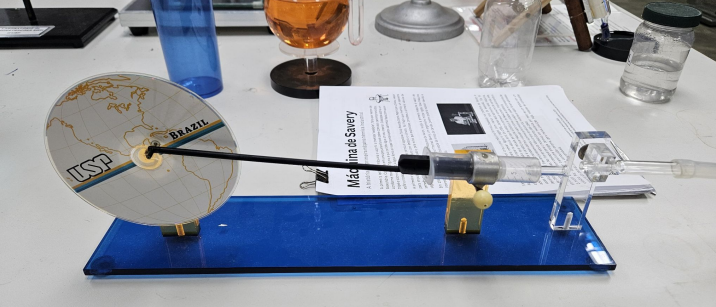
\includegraphics[width=0.45\linewidth]{fig/pistao.png}
\caption{Sistema pistão-dispositivo de giro movido por sopro. A imagem mostra o tubo de entrada de ar e o pistão conectado a um disco rotativo. Fonte: registro fotográfico feito pelo monitor Pedro.}
\label{fig:pistao}
\end{figure}

\subsection{Motor de Heron}
O dispositivo experimental foi composto por um reservatório de água conectado a tubos laterais abertos em formato de ``L''. Após ser aquecido, observou-se a liberação de vapor por esses tubos, criando movimento rotacionál. A montagem está ilustrada na \cref{fig:eron}.

\begin{figure}[H]
\centering
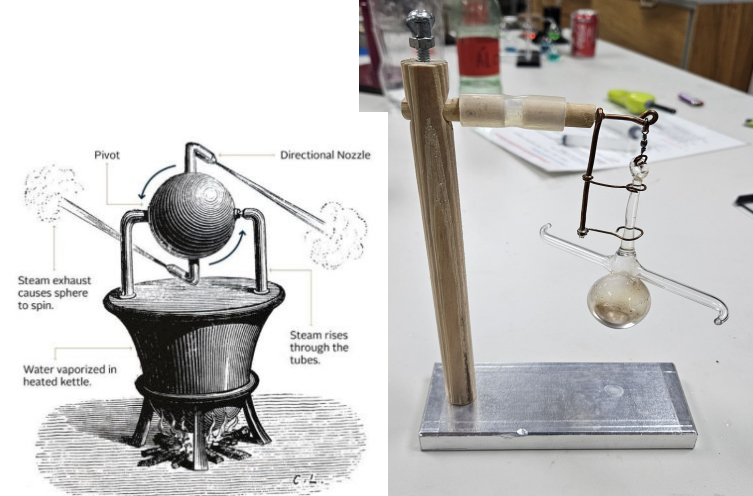
\includegraphics[width=0.42\linewidth]{fig/eron.png}
\caption{Montagem do motor de Heron. A imagem a direita mostra o sistema com tubos laterais por onde o vapor é liberado, enquanto a da direita mostra um representação gráfica do modelo. Fonte: imagens disponibilizadas pelo monitor da disciplina.}
\label{fig:eron}
\end{figure}

\subsection{Motor de Stirling}
Foram utilizados dois modelos distintos de motores de Stirling para observação do funcionamento mecânico. O primeiro modelo consistia em um cilindro metálico disposto horizontalmente, conectado a um pistão e a um volante de inércia, todos fixados sobre uma base rígida. O segundo modelo apresentava uma estrutura montada em base acrílica, composta por dois tubos verticais: um destinado ao suporte da fonte de calor e o outro acoplado a um bulbo de vidro contendo esferas no interior. Este bulbo encontrava-se ligado a um êmbolo com extremidade de borracha, capaz de realizar movimento alternado. Ambos os modelos foram posicionados sobre bancadas e submetidos ao aquecimento por fontes externas. A \cref{fig:stirling} mostra os sistemas utilizados.

\begin{figure}[H]
\centering
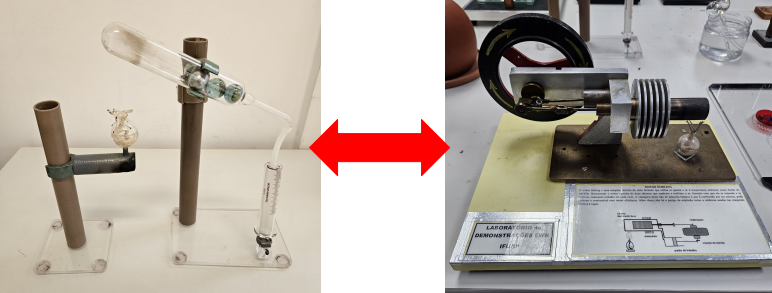
\includegraphics[width=0.55\linewidth]{fig/stirling.png}
\caption{Modelos experimentais de motores de Stirling: à esquerda, estrutura com tubos verticais, bulbo e êmbolo; à direita, sistema com cilindro metálico e volante de inércia. Fonte: fotografia feita pelo monitor da disciplina.}
\label{fig:stirling}
\end{figure}

\subsection{Máquina Térmica}
Foram utilizados dois modelos distintos de máquinas térmicas para fins de observação. O primeiro modelo consistia em uma representação esquemática, montada sobre uma base acrílica transparente. O sistema era composto por um conjunto de câmaras, pistão simulado, biela e volante, todos fixados com componentes coloridos para facilitar a visualização. O percurso do fluido de trabalho era indicado por setas na própria estrutura.
O segundo modelo tratava-se de uma máquina térmica funcional, montada com estrutura metálica e equipada com caldeira, pistão, biela, volante e uma correia conectada a um pequeno gerador. Durante o funcionamento, o calor gerado na caldeira movimentava o conjunto mecânico, acionando o gerador que, por sua vez, acendia um LED acoplado à estrutura, indicando a conversão de energia mecânica em energia elétrica. A \cref{fig:maquina} mostra os dispositivos utilizados.

\begin{figure}[H]
\centering
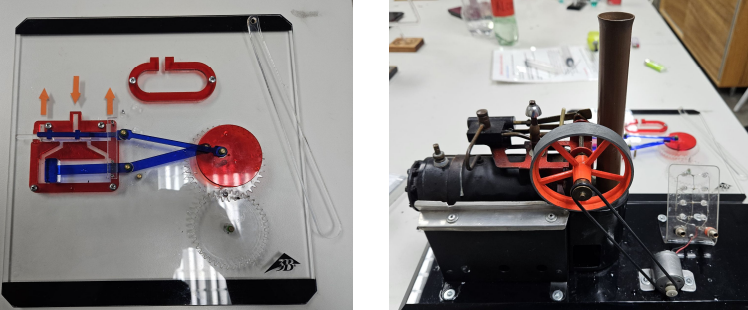
\includegraphics[width=0.55\linewidth]{fig/maquina.png}
\caption{Modelos de máquinas térmicas: à esquerda, representação esquemática em base acrílica com setas indicativas de fluxo; à direita, modelo funcional metálico com caldeira, volante e LED conectado ao gerador. Fonte: imagem capturada durante a aula por monitoria.}
\label{fig:maquina}
\end{figure}
